\section{Theorie}

    Im Folgenden werden die theoretischen Grundlagen der Strahlen- und Wellenoptik erläutert.\\
    \\
    Licht ist ein Teil des elektromagnetischen Wellenspektrums.
    Das für Menschen sichtbare Lichtspektrum umfasst die Wellenlängen
    von $\SI{380}{\nano\meter}$ bis $\SI{780}{\nano\meter}$,
    wobei das optische Spektrum bei $\SI{100}{\nano\meter}$ beginnt
    und bis hin zu $\SI{1}{\milli\meter}$ reicht.

\subsection{Strahlenoptik}

    In der Strahlenoptik wird die Ausbreitung der Lichtwellen über Wellenfronten und deren Normalen beschrieben.
    Die Lichtstrahlen breiten sich geradlinig aus und beeinflussen sich gegenseitig nicht.
    Beim Auftreffen einer Wellenfront auf eine Grenzfläche können nachfolgend beschriebenen Phänomene auftreten.
    Die Grenzfläche stellt eine Trennung zweier verschiedener Medien dar,
    deren Brechungsindizes mit $n_1$ und $n_2$ beschrieben werden.
    \autoref{fig:wellenfront} stellt dieses Szenario qualitativ dar.
    Die Faktoren $c_1$ und $c_2$ beschreiben in dieser Abbildung die Brechungsindizes.
    \begin{figure}[H]
        \centering
        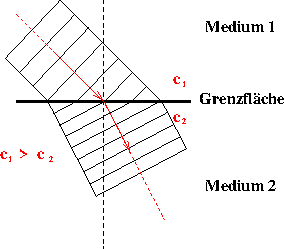
\includegraphics[width=0.5\textwidth]{content/img/Abb_1.pdf}
        \caption{Brechung einer Wellenfront an einer Grenzfläche zu einem anderen Medium. \cite{versuchsanleitung}}
        \label{fig:wellenfront}
    \end{figure}


\begin{description}
    \item[Reflexion]
    Bei der Reflexion trifft ein Lichtstrahl in einem Winkel $\alpha_1$ (gemessen zum Lot) auf die Grenzfläche
    und wird um den gleichen Winkel $\alpha_2$ reflektiert.
    Somit gilt:
    \begin{equation}
      \alpha_1 = \alpha_2 \ .
      \label{eqn:reflexionsgesetz}
    \end{equation}
    Dies ist in \autoref{fig:reflexion} dargestellt.

    \begin{figure}[H]
        \centering
        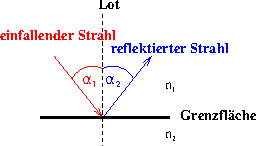
\includegraphics[width=0.5\textwidth]{content/img/Abb_2a.pdf}
        \caption{Reflexion eines Lichtstrahls an einer Grenzfläche. \cite{versuchsanleitung}}
        \label{fig:reflexion}
    \end{figure}


    \item[Brechung]
    Trifft ein Lichtstrahl auf eine Grenzfläche zwischen zwei Medien,
    so wird der Strahl \textit{gebrochen}.

    Beim Übergang von Luft mit dem Brechungsindex $n = \num{1.000292} \approx \num{1}$ in ein anderes Medium wird der Brechungsindex $n_2$ des Mediums als \textit{absoluter Brechungsindex} bezeichnet.
    Weiterhin wird unter Beobachtung der Ausbreitungsgeschwindigkeit $v$ der Wellen
    zwischen dem \textit{optisch dichteren} und dem \textit{optisch dünneren} Medium unterschieden.
    Wenn die Ausbreitungsgeschwindigkeit im Vergleich zu einem anderen Medium größer ist,
    wird dieses Medium als das optisch dichtere Medium bezeichnet.
    Wenn umgekehrt die Ausbreitungsgeschwindigkeit zu einem anderen Medium geringer ist,
    heißt dieses Medium optisch dünner.

    Ist das zweite Medium optisch dichter als das erste,
    wird der Strahl zum Lot hingebrochen,
    ist das erste Medium optisch dichter,
    wird der Strahl vom Lot weg gebrochen.

    Beim Übergang zwischen den Medien verändert sich die Ausbreitungsrichtung des Lichtstrahls,
    was in der \autoref{fig:brechung} dargestellt ist.

    \begin{figure}[H]
        \centering
        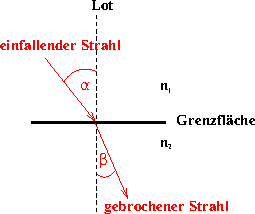
\includegraphics[width=0.5\textwidth]{content/img/Abb_2b.pdf}
        \caption{Brechung eines Lichtstrahls an einer Grenzfläche. \cite{versuchsanleitung}}
        \label{fig:brechung}
    \end{figure}

    Nach dem Snellius'schen Brechungsgesetz gilt beim Übergang zwischen den Medien
    \begin{align}
        \label{eqn:brechungsgesetz}
        \frac{\sin\alpha}{\sin\beta} &= \frac{v_1}{v_2} = \frac{n_2}{n_1}
        \intertext{was sich umformen lässt zu}
        \notag
        n_1 \sin\alpha &= n_2 \sin\beta \ .
    \end{align}
    Die Faktoren $v_1$ und $v_2$ beschreiben die Ausbreitungsgeschwindigkeit des Strahls im jeweiligen Medium.
    Die Ausbreitungsgeschwindigkeit in Luft beträgt $v = c = \SI{2.9979e8}{\meter\per\second}$.\\
    \\
    Für den Fall,
    dass der Strahl beim Übergang von einem Medium in ein zweites Medium gebrochen wird,
    sich in diesem weiterbewegt
    und beim Austritt zurück in das erste Medium wieder gebrochen wird,
    ergibt sich ein Strahlversatz $s$,
    welcher mit der Gleichung
    \begin{equation}
        s = d \; \frac{\sin(\alpha - \beta)}{\cos\beta}
        \label{eqn:strahlversatz}
    \end{equation}
    berechnet werden kann.
    Die beschriebene Situation ist in der folgenden Abbildung dargestellt.
    \begin{figure}[H]
        \centering
        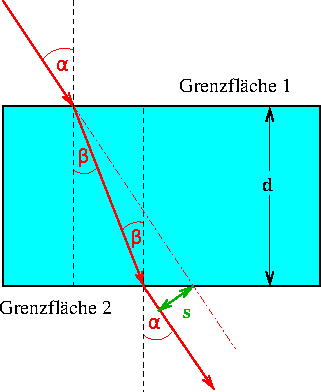
\includegraphics[width=0.4\textwidth]{content/img/Abb_5.pdf}
        \caption{Strahlversatz eines Lichtstrahls beim Durchqueren eines Mediums mit anderem Brechungsindex. \cite{versuchsanleitung}}
        \label{fig:strahlversatz}
    \end{figure}


    \item[Reflexion und Transmission]
    Tatsächlich wird ein Lichtstrahl beim Auftreffen auf eine Grenzfläche zum Teil reflektiert und gebrochen.
    Die Intensität des reflektierten Strahls wird mit $R$ bezeichnet,
    während die Intensität des transmittierten,
    gebrochenen Strahls mit $T$ bezeichnet wird.
    Die Größe von $R$ und $T$ ist materialabhängig,
    allerdings ist die Gesamtintensität stets erhalten:
    \[ R + T = 1 \ . \]

    In \autoref{fig:transmission} ist der Fall der Reflexion und Brechung, beziehungsweise Transmission dargestellt.
    \begin{figure}[H]
        \centering
        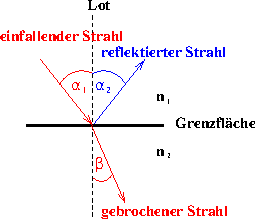
\includegraphics[width=0.5\textwidth]{content/img/Abb_2c.pdf}
        \caption{Reflexion und Brechung eines Lichtstrahls an einer Grenzfläche. \cite{versuchsanleitung}}
        \label{fig:transmission}
    \end{figure}
\end{description}


%\subsubsection{Reflexion}
%\subsubsection{Brechung}
%\subsubsection{Reflexion und Transmission}

\subsection{Wellenoptik}

    Zusätzlich zu den oben genannten Phänomenen kann ein Lichtstrahl an einem Hindernis \textit{gebeugt} werden,
    sodass sich das Licht auch im eigentlichen Schattenraum ausbreitet.
    Dies kann allerdings nur mit der Wellenoptik erklärt werden.\\
    \\
    Die Wellenoptik untersucht die Welleneigenschaften von Licht,
    wie die Amplitude, die Frequenz und die Wellenlänge.\\
    Für elektromagnetische Wellen gilt das Superpositionsprinzip,
    sodass sich die Amplituden zweier sich überlagender Wellen addieren,
    und sich eine Gesamtintensitätsverteilung ergibt.\\
    Unter der Bedingung der Kohärenz,
    also bei gleicher Frequenz und Polarisation sowie fester Phasenbeziehung,
    kann Licht Interferenzeffekte zeigen;
    es kommt, je nach Phasenverschiebung,
    zu konstruktiver oder destruktiver Interferenz.\\
    \\
    Für den Begriff der Beugung ist das Huygens'sche Prinzip relevant.
    Es sagt aus,
    dass jeder Punkt einer Wellenfront Ausgangspunkt einer neuen Elementarwelle mit gleicher Frequenz ist,
    wobei die Einhüllende der Elementarwellen eine neue Wellenfront ergibt.

    Nun wird ein Spalt der Breite $a$ betrachtet.
    Die Wellenfront,
    die auf den Spalt trifft,
    wird in jedem Punkt zu Wellen gleicher Frequenz und Phasenbeziehung gebeugt.
    Es ergibt sich ein Interferenzmuster.
    Die Betrachtung eines Spaltes kann auf ein Gitter mit $N$ Spalten erweitert werden.
    Für die Intensitätsmaxima $k$-ter Ordnung gilt:
    \begin{equation}
        d \cdot \sin\alpha = k \lambda \ .
        \label{eqn:intensitaetsmaxima}
    \end{equation}
    Die Größe $d$ stellt die Gitterkonstante dar;
    sie beschreibt,
    wie viele Spalte pro Millimeter das Gitter besitzt.


    Schließlich wird die Brechung an einem Prisma wie in \autoref{fig:prisma} betrachtet.
    \begin{figure}[H]
        \centering
        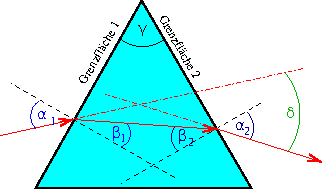
\includegraphics[width=0.5\textwidth]{content/img/Abb_6.pdf}
        \caption{Brechung eines Lichtstrahls an einem optische Prisma. \cite{versuchsanleitung}}
        \label{fig:prisma}
    \end{figure}
    Bei der Brechung am Prisma sind die Wellenlänge sowie die Ausbreitungsgeschwindigkeit des Lichts
    für die Brechungsverhältnisse relevant.

    Der Lichtstrahl wird beim Durchgang durch das Prisma abglenkt.
    Diese Ablenkung kann durch
    \begin{equation}
        \delta = (\alpha_1 + \alpha_2) - (\beta_1 + \beta_2)
        \label{eqn:ablenkung}
    \end{equation}
    bestimmt werden.
    \phantomsection
    \label{sec:theorie:dispersion}
    Der Brechungswinkel $\beta$ ist abhängig von der Wellenlänge,
    während der Einfallswinkel $\alpha$ beim Einfall von weißem Licht für alle Farben gleich ist.
    Die Abhängigkeit des Brechungswinkels von der Wellenlänge wird Dispersion genannt.
